\subsection{Population Size Inference}
\label{sec:population-size-inference}

Section \ref{sec:population-size-inference-principle} recaps the mechanistic principle behind distributed population size estimation and Section \ref{sec:population-size-inference-stats} reports statistical formulations derived to perform distributed population size estimation.
Section \ref{sec:ne-process-example} explains population size inference over an example evolutionary replicate.

Section \ref{sec:population-size-inference-experiments} describes the three treatments compared to test the proposed population size inference mechanism.

\subsubsection{Population Size Inference Principle}
\label{sec:population-size-inference-principle}

Consider a population composed of $n$ individuals, each holding a unique gene represented as an unsigned integer of a given precision.
At the outset, each gene value is assumed to be drawn from a uniform distribution across all possible values.
As generations evolve through sexual recombination, a ``gene drive'' mechanism is enforced where offspring inherit the larger gene value from their parents.
Over time, this mechanism results in the largest gene value becoming dominant or `fixed' in the population.

\begin{SCfigure}[3][b]
  \centering
  \begin{subfigure}[b]{0.4\textwidth}
    \centering
    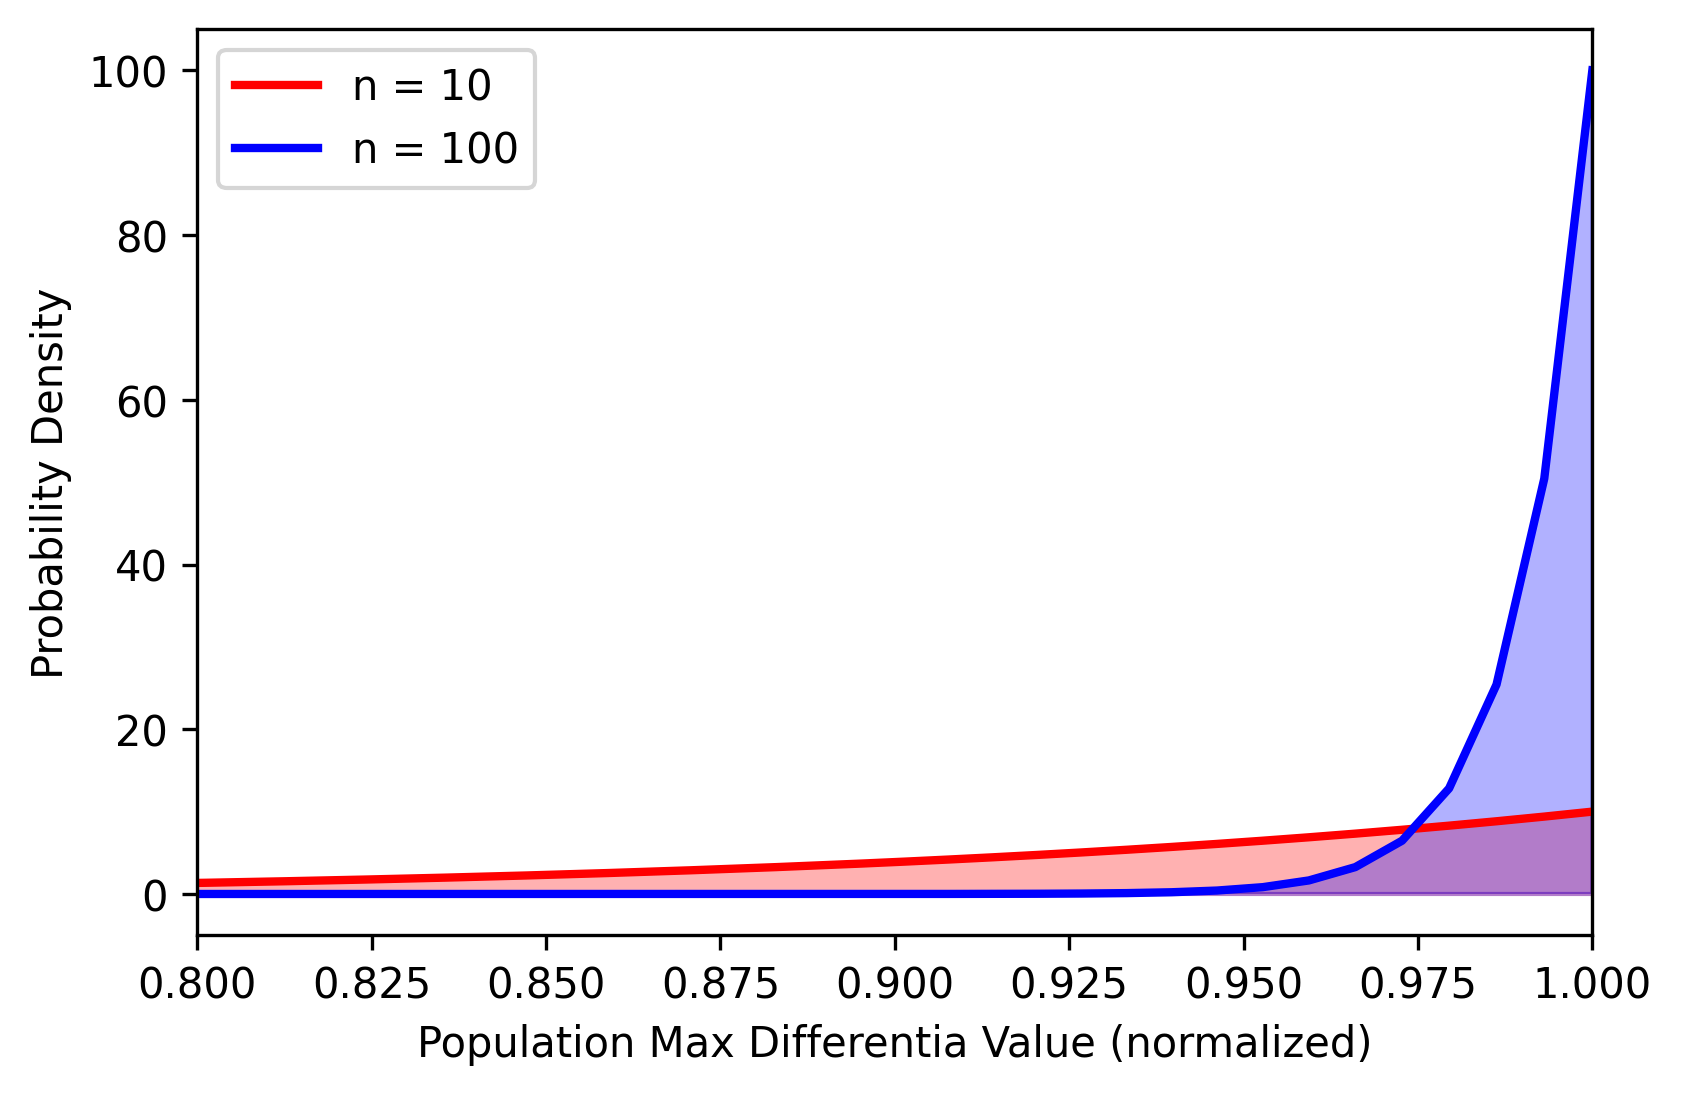
\includegraphics[width=\textwidth]{notebooks/notebooks/teeplots/viz=beta-pdf+ext=}
    % \caption{empty}
    % \label{fig:empty}
  \end{subfigure}%
  \begin{subfigure}[b]{0.25\textwidth}
    \centering
    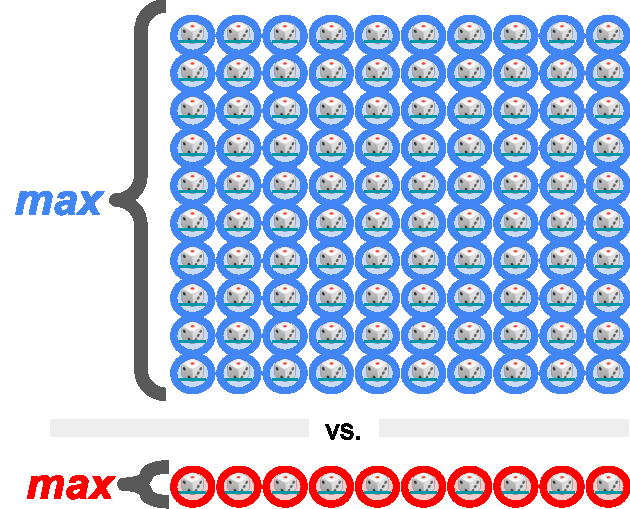
\includegraphics[width=\textwidth]{img/dice-pool}
    \vspace{2ex}
    % \caption{empty}
    % \label{fig:empty}
  \end{subfigure}
  \caption{
    Working principle of population size estimation.
    Increasing population size skews probability density function for population maximum value of generated fingerprints (referred to here as ``differentia'').
  }
  \label{fig:beta-explain}
\end{SCfigure}


An interesting property of this gene drive mechanism is the potential to estimate the original population size by observing the distribution of the fixed gene values.
By introducing a random variable $\mathbb{X}$ to represent the magnitude of the fixed gene value, we can explore its distribution.
Assuming our gene value is uniformly distributed between 0 and 1, it is identified as $\beta(n, 1)$ \citep{gentle2009computational} distributed.
Hence, by observing the values of these fixed genes, it's possible to infer $n$, the original population size (Figure \ref{fig:beta-explain}).
This approach is further extendable to cases involving multiple independent genes, each adhering to the same fixed precision and initial uniform distribution, providing a compelling estimation technique for population size.

Directly analogous techniques to estimate population size have also arisen in the context of decentralized, anonymous network engineering \citep{varagnolo2010distributed,hakan2012distributed}.
In these schemes, nodes independently draw a random vector of numerical values from a known distribution.
Values are exchanged through an aggregating function like (e.g., minimum, maximum, etc.), ultimately resulting in a consensus value fixing within the network.
Each node can then independently infer probabilistic information about the larger network, in a manner that is generally consistent across nodes.

\subsubsection{Population Size Inference Statistics}
\label{sec:population-size-inference-stats}

Statistical details necessary to work with the fixed-gene-magnitude inference method follow, some of which are, to best knowledge, not yet reported.
Derivations are available at \url{https://github.com/mmore500/hereditary-stratigraph-concept/tree/master/binder/popsize}, and will be included in supplemental material.

\paragraph{Maximum Likelihood Estimator}

The maximum likelihood estimator for population size given $i$ independent observations of fixed-gene magnitude $x_i$ is
\begin{align} \label{eqn:popsize_mle}
\hat{n}_\mathrm{mle} = -\frac{k}{\sum_{i=1}^k \log( x_i )}.
\end{align}

Mean square error of the maximum likelihood estimator for population size given $k$ observations of fixed gene magnitude is

\begin{align*}
n^2 \frac{k^{2}+ k-2}{(k-1)^{2}(k-2)}.
\end{align*}

These results were also derived in \citep{varagnolo2010distributed}.

\paragraph{Maximum Likelihood Estimator Expected Value}

Expected value for the maximum likelihood population size estimator $\hat{n}_\mathrm{mle}$ is given as

\begin{align*}
E(\hat{n}_\mathrm{mle})
= n\frac{k}{k-1}
\end{align*}

for $k>1$ \citep{varagnolo2010distributed}.
This value can be subtracted from the maximum likelihood estimator to yield a mean-unbiased population size estimator.

\paragraph{Confidence Interval}

Computation of confidence intervals is necessary of facilitate experimental inference from population size estimators.
Formulations derived from the maximum likelihood estimator are provided below.

For a single observation of fixed gene magnitude $\hat{x}$, the population size $n$ can be estimated with $c\%$ confidence to fall within the interval

\begin{align*}
\Big(
\frac{\log(\frac{1+c/100}{2})}{\log\hat{x}},
\frac{\log(\frac{1-c/100}{2})}{\log\hat{x}}
\Big).
\end{align*}

At this low observational power, the 95\% confidence interval spans a 145-fold order of magnitude and a 99\% confidence interval spans a 1057-fold order of magnitude.

For $k$ observations of fixed gene magnitude $\hat{x}_i$, the population size $n$ can be estimated with $c\%$ confidence to fall within the interval $(\hat{n}_\mathrm{lb}, \hat{n}_\mathrm{ub})$ where $\hat{n}_\mathrm{lb}$ is the solution to

\begin{align} \label{eqn:popsize_mle_ci_lb}
0
&= 2\Gamma\Big(k, -\hat{n}_\mathrm{lb}\log(\prod_{i=1}^k\hat{x}_i)\Big) - (c/100+1)\Gamma(k)
\end{align}

and $\hat{n}_\mathrm{ub}$ is the solution to

\begin{align} \label{eqn:popsize_mle_ci_ub}
  0
  &= 2\Gamma\Big(k, -\hat{n}_\mathrm{ub}\log(\prod_{i=1}^k\hat{x}_i)\Big) - (1-c/100)\Gamma(k).
\end{align}

Here, $\Gamma$ is the complete gamma function.

Four independent observations are sufficient to provide a 95\% confidence interval spanning 8-fold magnitude or a 99\% confidence interval spanning a 16-fold magnitude.
Nine independent observations are sufficient for a 95\% confidence interval spanning a factor spanning 4-fold magnitude or a 99\% confidence interval spanning a factor of 6-fold magnitude.
33 independent observations are sufficient for a 95\% confidence interval spanning 2-fold magnitude or a 99\% confidence interval spanning 2.5-fold magnitude.

Note that the width of the confidence interval will scale as a constant factor of as $n \to \infty$.

\paragraph{Median-unbiased Estimator}

A median-unbiased estimator $\hat{n}_\mathrm{mle}$ for population can be trivially derived from the confidence interval, as the numerical solution of

\begin{align*}
0
&= 2\Gamma\Big(k, -\hat{n}_\mathrm{mumle}\log(\prod_{i=1}^k x_i)\Big) - \Gamma(k).
\end{align*}

\paragraph{Credible Intervals}

Computation of credible intervals facilitates bayesian inference from estimators.
Derivation assumes a uniform prior over population size.
The credibility contained within a factor $f$ of the maximum likelihood estimate $\hat{n}_\mathrm{mle}$ can be calculated as


\begin{align*}
\frac{- \gamma(k + 1, \frac{k}{f}) + \gamma(k + 1, f k)}{k!}.
\end{align*}

Here, $\gamma$ is the lower incomplete gamma function.

By its form, the credibility contained within a factor of maximum likelihood estimate remains constant across population sizes $n$.
Credibility intervals require similar sample sizes to provide $n$-fold magnitude spans as those for confidence intervals discussed above.

\paragraph{Rolling Population Size Estimation} \label{sec:rolling_estimation}

Experiments reported here use a simple rolling process to aggregate ten preceding fixed-gene magnitudes to compute a population size estimate and confidence intervals.
More sophisticated regularizations have been proposed to consolidate time series estimates of dynamically-changing network sizes \citep{hakan2012distributed}.

\subsubsection{Example Population Size Inference}
\label{sec:ne-process-example}

\begin{figure}
  \centering

  \begin{minipage}{.65\textwidth}
    \centering
    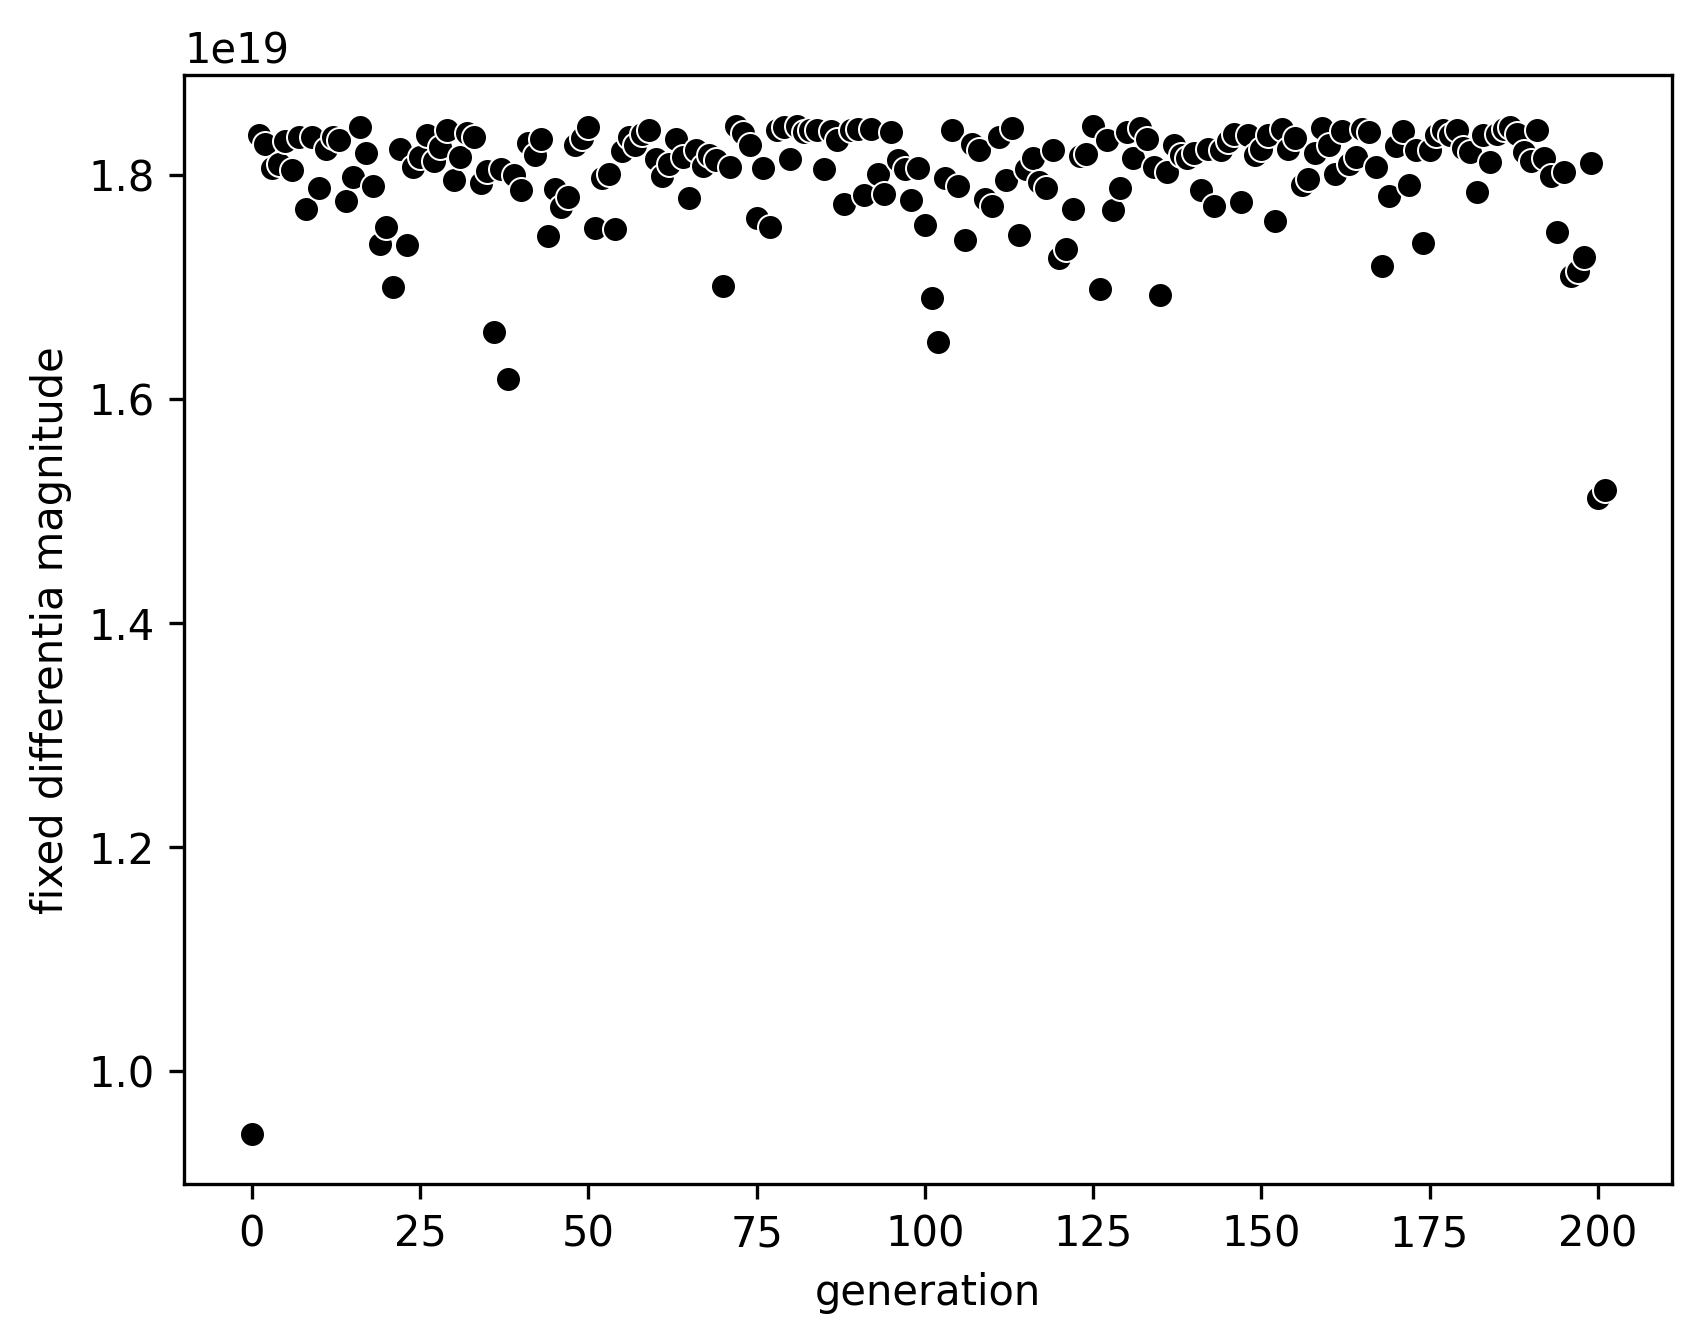
\includegraphics[height=0.25\textheight]{notebooks/notebooks/teeplots/notebook=ne-inference+replicate=0+treatment=control+viz=scatterplot-differentia-magnitude+ext=}
  \end{minipage}%
  \begin{minipage}{.25\textwidth}
    \subcaption{Fixed Species-level Differentia Magnitudes by Layer}
    \label{fig:ne-process-example:differentia}
  \end{minipage}

  \vspace{0.25em}

  \begin{minipage}{.65\textwidth}
    \centering
    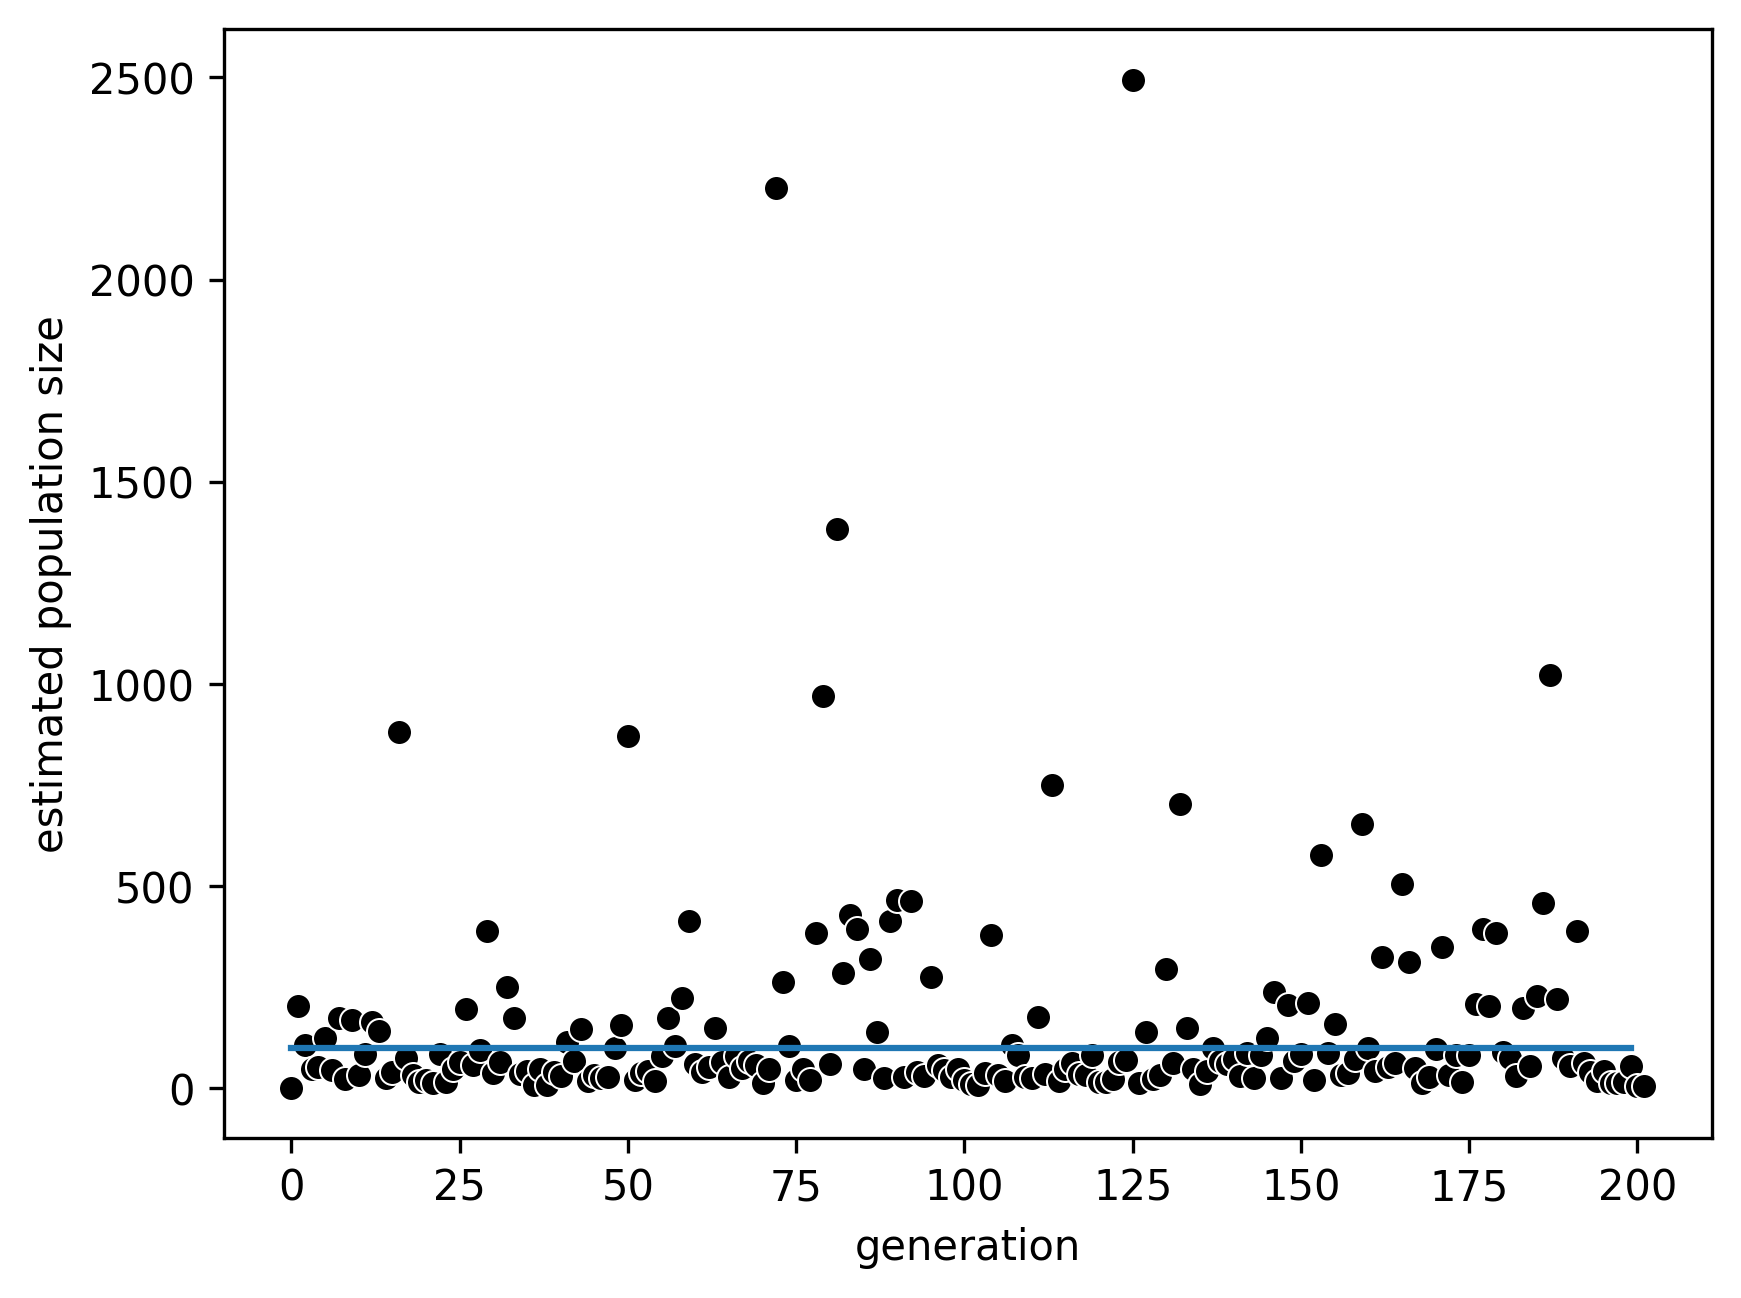
\includegraphics[height=0.25\textheight]{notebooks/notebooks/teeplots/notebook=ne-inference+replicate=0+treatment=control+viz=scatterplot-popsize-estimates+ext=}
  \end{minipage}%
  \begin{minipage}{.25\textwidth}
    \subcaption{Population Size Estimates}
    \label{fig:ne-process-example:singleton-est}
  \end{minipage}

  \vspace{0.25em}

  \begin{minipage}{.65\textwidth}
    \centering
    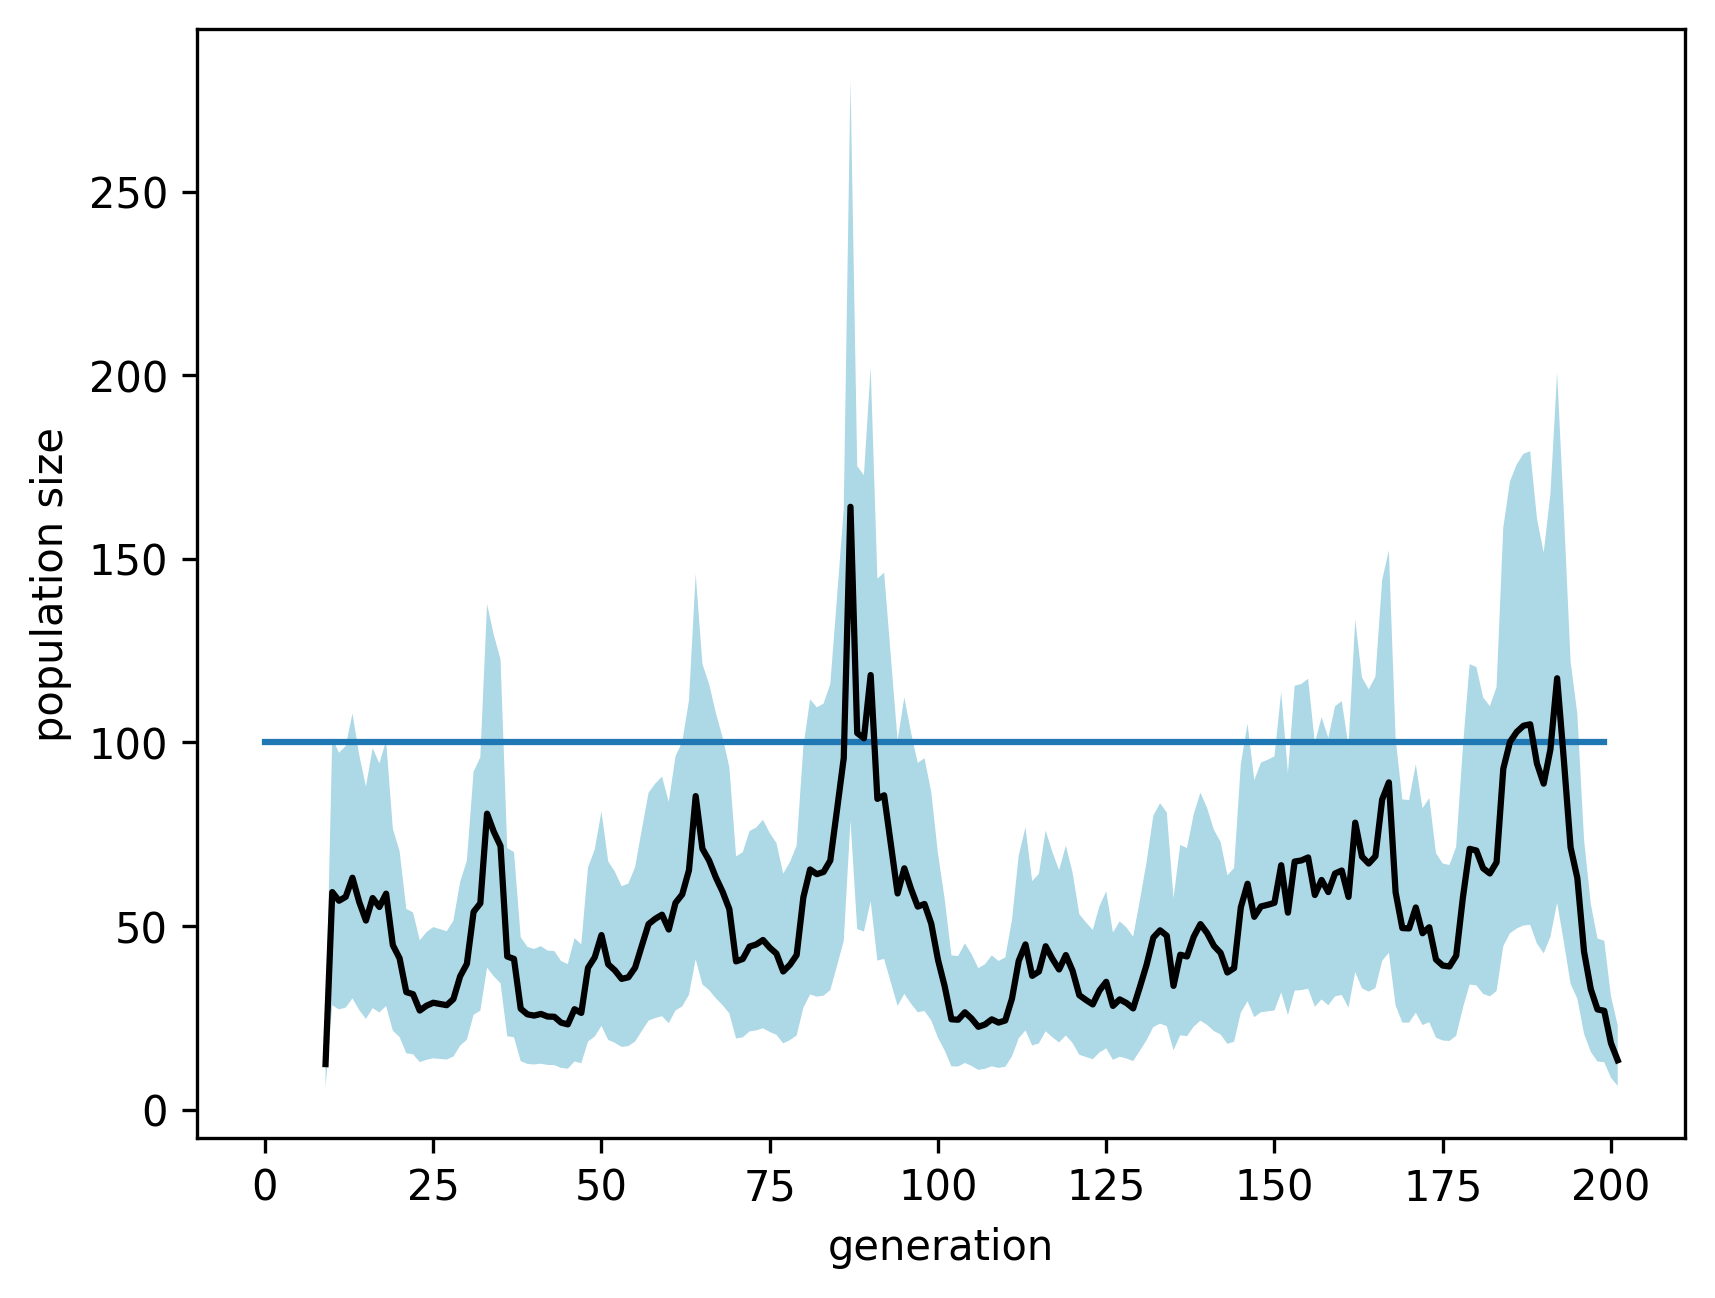
\includegraphics[height=0.25\textheight]{notebooks/notebooks/teeplots/notebook=ne-inference+replicate=0+treatment=control+viz=plot-running-estimation+x=rank+y=population-size+ext=}
  \end{minipage}%
  \begin{minipage}{.25\textwidth}
    \subcaption{Running Population Size Estimation with 95\% Confidence Intervals}
    \label{fig:ne-process-example:running-est}
  \end{minipage}

  \caption{
    Example population size estimation data.
    Differentia values are extracted from species-level annotation of a single extant population member (Subfigure \ref{fig:ne-process-example:differentia}).
    Subfigure \ref{fig:ne-process-example:singleton-est} shows one-off population size estimates at each generation from the corresponding differentia.
    To improve statistical informativeness, differentia values are grouped into a running pool of ten values to perform population size estimation.
    True population carrying capacity is annotated as a horizontal line.
    Note that systematic underestimation of ``carrying capacity'' population size is expected due to demographic factors excluding some population members from gene pool contributions.
    Figure \ref{fig:beta-explain} overviews the statistical mechanism used for population size distribution.
  }
  \label{fig:ne-process-example}
\end{figure}


% notebooks/notebooks/teeplots/notebook=ne-inference+replicate=0+treatment=control+viz=plot-running-estimation+x=rank+y=population-size+ext=.pdf
%
% notebooks/notebooks/teeplots/notebook=ne-inference+replicate=0+treatment=control+viz=scatterplot-differentia-magnitude+ext=.pdf
%
% notebooks/notebooks/teeplots/notebook=ne-inference+replicate=0+treatment=control+viz=scatterplot-popsize-estimates+ext=.pdf


% notebooks/notebooks/teeplots/notebook=ne-inference+replicate=0+treatment=bottleneck+viz=plot-running-estimation+x=rank+y=population-size+ext=.pdf
%
% notebooks/notebooks/teeplots/notebook=ne-inference+replicate=0+treatment=bottleneck+viz=scatterplot-differentia-magnitude+ext=.pdf
%
% notebooks/notebooks/teeplots/notebook=ne-inference+replicate=0+treatment=bottleneck+viz=scatterplot-popsize-estimates+ext=.pdf

% notebooks/notebooks/teeplots/notebook=ne-inference+replicate=0+treatment=range-expansion+viz=plot-running-estimation+x=rank+y=population-size+ext=.pdf
%
% notebooks/notebooks/teeplots/notebook=ne-inference+replicate=0+treatment=range-expansion+viz=scatterplot-differentia-magnitude+ext=.pdf
%
% notebooks/notebooks/teeplots/notebook=ne-inference+replicate=0+treatment=range-expansion+viz=scatterplot-differentia-magnitude+ext=.pdf
%
% notebooks/notebooks/teeplots/notebook=ne-inference+replicate=0+treatment=selection-pressure+viz=plot-running-estimation+x=rank+y=population-size+ext=.pdf
%
% notebooks/notebooks/teeplots/notebook=ne-inference+replicate=0+treatment=selection-pressure+viz=scatterplot-differentia-magnitude+ext=.pdf
%
% notebooks/notebooks/teeplots/notebook=ne-inference+replicate=0+treatment=selection-pressure+viz=scatterplot-popsize-estimates+ext=.pdf


Figure \ref{fig:ne-process-example} shows an example of population size inference over the course of an experiment.

Panel \ref{fig:ne-process-example:differentia} shows magnitudes of fixed differentia across the generational record extracted from a sample specimen at the end of the run.

Population size estimates can be computed at each generation using the maximum likelihood estimator (Equation \ref{eqn:popsize_mle}, as shown in Panel \ref{fig:ne-process-example:singleton-est}.
The true population size is annotated as a horizontal blue line.

To generate more robust inference, inference was pooled over rolling sets of 10 fixed differentia.
Population size estimates were again performed using Equation \ref{eqn:popsize_mle} with confidence interval bounds computed from Equations \ref{eqn:popsize_mle_ci_lb} and \ref{eqn:popsize_mle_ci_ub}.
Figure \ref{fig:ne-process-example:running-est} plots this running estimation.
Note that some discrepancy is expected between absolute population size (horizontal line) and effective population size $N_e$ (estimated) due to demographic factors.

\subsubsection{Population Size Inference Experiment}
\label{sec:population-size-inference-experiments}

The experiment tested the ability of the population size estimation process (Section \ref{sec:ne-process-example} to detect effective population size differences between populations and effective population size changes within a population over time.
Four different treatment conditions were compared: bottleneck, range expansion, selection pressure, and control.
Ten independent replicates were performed for each treatment.

The bottleneck treatment simulated a population reduction event.
The population size was kept at 100 for 67 generations, reduced an order of magnitude to 10 for 66 generations, and then returned to 100 for another 67 generations.

The range expansion treatment simulated gradual population size expansion.
The population size was initiated at at 10 for 67 generations, then increased linearly for 66 generations to 142 at generation 133, and then maintained at 142 for another 67 generations.

The selection-pressure treatment modified the selection intensity during the evolutionary process.
This reduced the effective population size by increasing the number of population members eliminated without contributing to the next generation. gene pool.
High selection pressure was applied for 67 generations (tournament size 8). Then, selection pressure was eliminated for 66 generations (tournament size of 1).
Finally, high selection pressure (tournament size 8) was reinstated for the last 67 generations.

The control treatment was run with a constant population size of 100 for 200 generations.
